\documentclass[usenames,dvipsnames,aspectratio=169]{beamer}
\usepackage{../common/web}

\title[Web technológiák - HTML]{Web-technológia}
\subtitle{HTML, II. rész}

\begin{document}

%1
\begin{frame}[plain]
  \titlepage
  \logoalul
\end{frame}

\section{HTML5}

\subsection{Űrlapok}

%86
\begin{frame}
  Vastag kliens alkalmazásokhoz hasonlóan adatok gyűjthetőek űrlapokkal, amiket 
  \begin{itemize}
    \item feldolgoztathatunk a szerver oldalon (most ez lesz), vagy
    \item JavaScript programmal a kliensen.
  \end{itemize}
  Űrlap vezérlők a \texttt{<form>} elembe ágyazva használhatók. Legfontosabb attribútumai:
  \begin{description}[m]
    \item[\texttt{action}] \hfill \\ A szerver oldali feldolgozó script URL-je
    \item[\texttt{target}] \hfill \\ Hova töltse a szerver válaszát 
    (\texttt{\_blank}, \texttt{\_self} (alapért.), \texttt{\_parent}, \dots)
    \item[\texttt{novalidate}] \hfill \\ Ne végezzen input 
    ellenőrzést a böngésző
    \item[\texttt{autocomplete}] \hfill \\ Korábban megadottak alapján 
    kiegészíti az adatokat (\texttt{on} (alapért.), \texttt{off})
  \end{description}
\end{frame}

%87
\begin{frame}
  \begin{description}[m]
    \item[\texttt{method}] \hfill \\ Adattovábbítási módszer:
    \begin{description}[m]
      \item[\texttt{get}] \hfill \\ Alapértelmezett. URL lekérdező 
      karakterláncában továbbítja az adatokat.
      \begin{itemize}
        \item Az URL betehető a könyvjelzők közé, és
        \item a böngészőben is könnyen szerkeszthető
      \end{itemize}
      \item[\texttt{post}] \hfill \\ HTTP tranzakcióként továbbít.
      \begin{itemize}
        \item Nincsenek méretkorlátok (URL hossza korlátozott, 
        $\approx$ 2000 karakter)
        \item Fájlok csak így továbbíthatók
        \item A böngészőben nem látszik, de ettől még \kiemel{nyílt 
        szöveg}ként továbbítják a hálózaton!
      \end{itemize}
    \end{description}
  \end{description}
\end{frame}

%88
\begin{frame}
  \begin{description}[m]
    \item[\texttt{enctype}] (type of encoding) \hfill \\ Meghatározza 
    a küldött adatok kódolását. Kötelező megadni, ha a \texttt{method} 
    attr. értéke \texttt{post}. Lehetséges értékek:
    \begin{description}[m]
      \item[\texttt{application/x-www-form-urlencoded}] \hfill \\ 
      Alapértelmezett. Minden szóközt és speciális karaktert 
      helyettesít.
      \item[\texttt{multipart/form-data}] \hfill \\ Fájlok küldésekor 
      kell használni.
      \item[\texttt{\texttt{text/plain}}] \hfill \\ Csak a szóközöket 
      helyettesíti.
    \end{description}
  \end{description}
\end{frame}

%89
\begin{frame}
  A legtöbb vezérlő az \texttt{<input>} elemmel hozható létre, pl. 
  egy számbeviteli mező néhány attribútuma, és hatása:
  \begin{description}[m]
    \footnotesize
    \item[\texttt{type}] \hfill \\ \texttt{number}, számbeviteli mező 
    létrehozása
    \item[\texttt{name}] \hfill \\ A szerver oldalon ez lesz az adat 
    \emph{kulcsa}
    \item[\texttt{min}] \hfill \\ A legkisebb bevihető érték
    \item[\texttt{max}] \hfill \\ A legnagyobb bevihető érték
    \item[\texttt{step}] \hfill \\ Ennyit változtatnak a 
    léptetőgombok/kurzurvezérlő nyilak az értéken, ennyi 
    többszöröseit lehet megadni, illetve ha 
    értéke \texttt{any}, akkor bármilyen racionális szám megadható
    \item[\texttt{required}] \hfill \\ A mező kitöltése kötelező
  \end{description}
\end{frame}

%90
\begin{frame}
  Űrlapbeküldő gomb: \texttt{<input>} elem
  \begin{itemize}
    \item \texttt{type="submit"}
    \item \texttt{value} attr. adja meg a gomb feliratát
  \end{itemize}
  \vfill
  Cimke létrehozása vezérlőhöz: \texttt{<label>} elemmel. A 
  cimkére kattintva a vezérlő is aktiválódik (pl. rádiógombnál 
  kiválasztás). Kapcsolat cimke és 
  vezérlő között:
  \begin{itemize}
    \item vezérlő a cimke belsejébe ágyazva
    \item a cimke \texttt{for} attribútumában megadható a vezérlő 
    \texttt{id}-je
  \end{itemize}
\end{frame}

%91
\begin{frame}
  Vezérlők logikai csoportosítása: \texttt{<fieldset>} elemmel\\
  Csoport feliratának megadása: \texttt{<legend>} elemben
  \vfill
  \begin{center}
    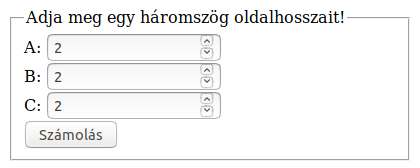
\includegraphics[width=.5\textwidth]{urlap1.png}
  \end{center}
\end{frame}

%92
\begin{frame}
  \begin{exampleblock}{\textattachfile{urlap1.html}{urlap1.html} 
  (\textattachfile{urlap1.php}{urlap1.php})}
    \footnotesize
    \lstinputlisting[style=HTML,linerange={8-20},numbers=left,firstnumber=8]{urlap1.html}
  \end{exampleblock}
\end{frame}

%93
\begin{frame}
  A legtöbb vezérlő az \texttt{<input>} elemmel és annak \texttt{type} 
  attribútumával állítható elő. Az összes vezérlővel használható főbb 
  attribútumai: 
  \begin{description}[m]
    \item[\texttt{autocomplete}] \hfill \\ Automatikus kiegészítés a 
    korábban begépelt tartalom alapján. (\texttt{on}, \texttt{off}) 
    \item[\texttt{autofocus}] \hfill \\ Oldalbetöltés után 
    automatikusan fókuszba kerül 
    \item[\texttt{disabled}] \hfill \\ Letiltott vezérlő 
    \item[\texttt{form}] \hfill \\ Ha a vezérlő 
    nincs \texttt{<form>} elembe ágyazva, akkor annak \texttt{id}-je 
    alapján logikailag összekapcsolható vele.
  \end{description}
\end{frame}

%94
\begin{frame}
  \begin{description}[m]
    \item[\texttt{id}] \hfill \\ A vezérlőt egyedileg azonosítja a 
    \kiemel{kliens} oldalon (pl. JavaScript programokban)
    \item[\texttt{name}] \hfill \\ A vezérlőt azonosítja a 
    \kiemel{szerver} oldalon (kulcs) 
    \item[\texttt{readonly}] \hfill \\ Csak olvashatóvá teszi a vezérlőt 
    \item[\texttt{required}] \hfill \\ A mező kitöltése kötelező 
    \item[\texttt{value}] \hfill \\ A vezérlő értéke
  \end{description}
\end{frame}

%95
\begin{frame}
  Egysoros szövegbeviteli mező: \texttt{type="text"} (alapértelmezés)
  \begin{description}[m]
    \item[\texttt{list}] \hfill \\ Egy \texttt{<datalist>} elem (ajánlatok legördülő listája) \texttt{id}-jét tartalmazza
    \item[\texttt{maxlength}] \hfill \\ A begépelhető karakterek száma
    \item[\texttt{pattern}] \hfill \\ Reguláris kifejezés az érték ellenőrzéséhez. Hiba esetén a \texttt{title} értéke magyarázza az elvárt formátumot.
    \item[\texttt{placeholder}] \hfill \\ Helyőrző, ami az első karakter begépeléséig segít a felhasználónak, pl. ,,A rendszámot kötőjel nélkül, nagybetűkkel adja meg!''
    \item[\texttt{size}] \hfill \\ A vezérlő szélessége átlagos karakterszélességben mérve (CSS jobb)
  \end{description}
\end{frame}

%96
\begin{frame}
  A \texttt{<datalist>} elembe \texttt{<option>} elemek ágyazhatók, 
  melyek gépelést segítő legördülő lista elemeiként jelennek meg.\\
  A (\texttt{<select>} elemben is használható) \texttt{<option>} attribútumai:
  \begin{description}[m]
    \item[\emph{attribútum nélkül}] \hfill \\ Az elem tartalma jelenik meg a legördülő listában, és ezt továbbítják a szervernek is
    \item[\texttt{label}] \hfill \\ A listában egy rövidebb szöveg jelenhet meg, mint az elem értéke
    \item[\texttt{selected}] \hfill \\ Kiválasztottá teszi az elemet az oldal betöltésekor (csak \texttt{<select>-nél})
    \item[\texttt{value}] \hfill \\ Ha megadják, ennek tartalmát küldi a szervernek (vagy másolja a szövegmezőbe), nem a megjelenő szöveget
  \end{description}
\end{frame}

%97
\begin{frame}
  Reguláris kifejezések dióhéjban\\
  \vfill
  Általános forma: \texttt{/\kiemel{minta}/módosítók}\\
  Input ellenőrzésre csak a \texttt{minta} szolgál; ha a vezérlő értéke nem illeszkedik az általános mintára, az űrlapot nem lehet beküldeni.\\
  \begin{itemize}
    \item Az általános karakterek önmagukat reprezentálják.
    \item A metakarakterek önmagukban is halmazt vagy vezérlőjelet testesítenek meg, pl. \texttt{\textbackslash d} a számjegyek, \texttt{\textbackslash s} a fehér karakterek, \texttt{\textbackslash n} az újsor, stb.
    \item Halmaz elemei közül elég egynek illeszkednie, pl. \texttt{[abc]} elfogadja az abc első három betűje közül bármelyiket.
    \item Halmaz intervallummal is megadható, pl. \texttt{[a-z]} a kisbetűk halmaza, de a két módszer kombinálható is, pl. \texttt{[a-zA-Z]} a betűk halmaza.
    \item Az \texttt{[\textasciicircum abc]} minden jelre illeszkedik, ami nem \texttt{a}, \texttt{b}, és \texttt{c}.
    \item Alternatívák is létrehozhatók \texttt{(a|b)} formában.
  \end{itemize}  
\end{frame}

%98
\begin{frame}
  Mennyiségek szabályozása
  \medskip
  \begin{itemize}
    \item \texttt{n+} legalább egy előfordulást vár el
    \item \texttt{n*} 0 vagy több előfordulást követel
    \item \texttt{n?} 0 vagy 1 előfordulás
    \item \texttt{n\{X\}} pontosan X előfordulás
    \item \texttt{n\{X,Y\}} legalább X, legfeljebb Y előfordulás
    \item \texttt{n\{X,\}} legalább X előfordulás
  \end{itemize}
  Pl. egy rendszámot ellenőriz a \texttt{[A-Za-z]\{3\}-\textbackslash d\{3\}} minta. 
  \hiv{\href{http://html5pattern.com/}{További minták.}}
  \vfill
  \hiv{\href{https://developer.mozilla.org/en-US/docs/Web/JavaScript/Guide/Regular_Expressions}{További részletek}}
\end{frame}

%99
\begin{frame}
  \begin{center}
    
\includegraphics[width=.5\textwidth]{urlap2-1.png}\\\vspace{-.5cm}\hrulefill\\
    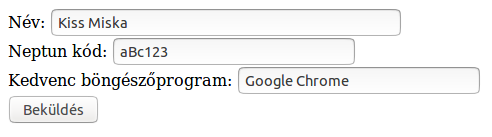
\includegraphics[width=.5\textwidth]{urlap2-2.png}\\\vspace{-.5cm}\hrulefill\\
    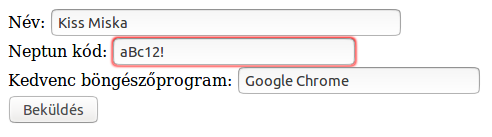
\includegraphics[width=.5\textwidth]{urlap2-3.png}\\
  \end{center}
\end{frame}

%100
\begin{frame}
  \begin{exampleblock}{\textattachfile{urlap2.html}{urlap2.html} (\textattachfile{urlap2.php}{urlap2.php})}
    \footnotesize
    \lstinputlisting[style=HTML,linerange={9-15},numbers=left,firstnumber=9]{urlap2.html}
  \end{exampleblock}
\end{frame}

%101
\begin{frame}
  \begin{exampleblock}{\textattachfile{urlap2.html}{urlap2.html} (\textattachfile{urlap2.php}{urlap2.php})}
    \footnotesize
    \lstinputlisting[style=HTML,linerange={16-25},numbers=left,firstnumber=16]{urlap2.html}
  \end{exampleblock}
\end{frame}

%102
\begin{frame}
  Jelszóbeviteli mező: \texttt{type="password"}\\
  Nagyon hasonló a \texttt{text} típushoz, de a karaktereket ,,elrejti'' (viszont \kiemel{nem titkosítja}!)
  \vfill
  Színválasztó: \texttt{type="color"}\\
  A \texttt{value} értéke \texttt{\#RRGGBB} formátumú.
  \vfill
  Dátumválasztó: \texttt{type="date"}\\
  A \texttt{value} értéke \emph{éééé-hh-nn} formátumú. Használhatóak még a \texttt{min}, \texttt{max} attribútumok.
  \vfill
  Dátum és időválasztó (időzóna nélkül):  \texttt{type="datetime-local"}\\
  A \texttt{value} értéke \emph{éééé-hh-nnTóó:pp} formátumú.
\end{frame}

%103
\begin{frame}
  E-mail cím megadása: \texttt{type="email"}\\
  Automatikusan ellenőrzi formailag. Több cím is megadható vesszőkkel elválasztva, ha megadják a \texttt{multiple} attribútumot.
  \vfill
  Rejtett mező: \texttt{type="hidden"}\\
  Egyáltalán nem jelenik meg, de egy (pl. JavaScript kóddal előállított) kulcs 
  (\texttt{name}) - érték (\texttt{value}) pár felküldhető a szerverre.
  \vfill
  Fájlok feltöltése: \texttt{type="file"}\\
  Több fájl feltölthető a \texttt{multiple} attribútum megadásával. 
  Korlátozható a tallózható fájlok köre, pl. \texttt{accept=".jpg"} csak 
  JPEG fájlokat enged, egy MIME-típus, mint pl. a \texttt{accept="video/*"} 
  mindenféle videót, stb. Korlátozható a fájlok mérete is:\\
  \texttt{<input type="hidden" name="MAX\_FILE\_SIZE" value="\emph{méret}" />}\\
  A kódolás típusa legyen \texttt{enctype="multipart/form-data"}, a HTTP 
  metódus \texttt{method="POST"}!
\end{frame}

%104
\begin{frame}
  \begin{center}
    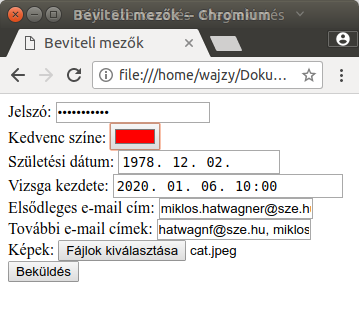
\includegraphics[width=.5\textwidth]{urlap3.png}
  \end{center}
\end{frame}

%105
\begin{frame}
  \begin{exampleblock}{\textattachfile{urlap3.html}{urlap3.html} (\textattachfile{urlap3.php}{urlap3.php})}
    \footnotesize
    \lstinputlisting[style=HTML,linerange={8-17},numbers=left,firstnumber=8]{urlap3.html}
  \end{exampleblock}
\end{frame}

%106
\begin{frame}
  \begin{exampleblock}{\textattachfile{urlap3.html}{urlap3.html} (\textattachfile{urlap3.php}{urlap3.php})}
    \footnotesize
    \lstinputlisting[style=HTML,linerange={18-27},numbers=left,firstnumber=18]{urlap3.html}
  \end{exampleblock}
\end{frame}

%107
\begin{frame}
  \begin{exampleblock}{Készítse el az alábbi űrlapot! (\textattachfile{urlap4.html}{urlap4.html})}
    Az adatokat küldje a \texttt{http://xenia.sze.hu/\textasciitilde wajzy/html/urlap3.php} címre!
    \begin{columns}[T]
      \column{0.45\textwidth}
        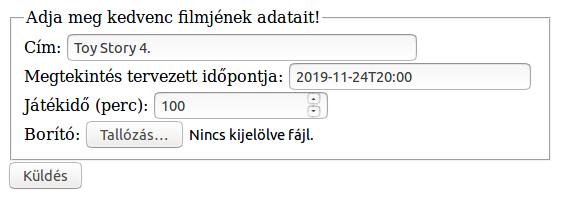
\includegraphics[width=\textwidth]{urlap4-1.png}
      \column{0.45\textwidth}
        
\includegraphics[width=\textwidth]{urlap4-2.png}
    \end{columns} 
  \end{exampleblock}
\end{frame}

%108
\begin{frame}
  Év és hónap kiválasztás: \texttt{type="month"}\\
  A \texttt{value} értéke \emph{éééé-hh} formátumú. Használhatóak még a \texttt{min}, \texttt{max} attribútumok.
  \vfill
  Év és azon belül egy hét kiválasztása: \texttt{type="week"}\\
  A \texttt{value} értéke \emph{éééé-Whh} formátumú.
  \vfill
  Idő megadása: \texttt{type="time"}\\
  A \texttt{value} értéke \emph{óó:pp} formátumú.
  \vfill
  Nyomógomb: \texttt{type="button"}\\
  Önmagában semmire nem jó, JavaScript kódok futtatására használják.
  \vfill
  Űrlap alaphelyzetbe állítása: \texttt{type="reset"}\\
  Az űrlap betöltése utáni állapotot állítja vissza; ha véletlenül kattintanak rá, minden addigi munka elvész!
\end{frame}

%109
\begin{frame}
  Jelölőnégyzet: \texttt{type="checkbox"}\\
  Egymástól független választási lehetőségekhez. 
  \vfill
  Rádiógomb: \texttt{type="radio"}\\
  Egy rádiógomb-csoporton belül csak egy elem lehet kiválasztva. 
  A felhasználó nem tudja az összes elemet ki nem választottá 
  tenni. Csoportképző módszer: azonos \texttt{name} attribútum 
  értékek.
  \vfill
  Mindkét típusra igaz, hogy egy elemet kiválasztani a 
  \texttt{checked} attribútummal lehet. A \texttt{value} attribútumot rádiógomboknál 
  ,,kötelező'' megadni, mert különben csak az \texttt{on} értéket 
  kapja meg a szerver $\to$ a gomb azonosíthatatlan. A ki nem 
  választott elemeknek még a kulcsa sem látszik a szerveren.
\end{frame}

%110
\begin{frame}
  \begin{center}
    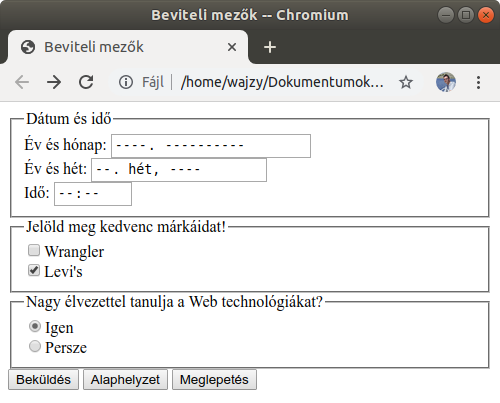
\includegraphics[width=.5\textwidth]{urlap5.png}
  \end{center}
\end{frame}

%111
\begin{frame}
  \begin{exampleblock}{\textattachfile{urlap5.html}{urlap5.html}}
    \footnotesize
    \lstinputlisting[style=HTML,linerange={11-16},numbers=left,firstnumber=11]{urlap5.html}
    \lstinputlisting[style=HTML,linerange={19-23},numbers=left,firstnumber=19]{urlap5.html}
  \end{exampleblock}
\end{frame}

%112
\begin{frame}
  \begin{exampleblock}{\textattachfile{urlap5.html}{urlap5.html}}
    \footnotesize
    \lstinputlisting[style=HTML,linerange={27-30},numbers=left,firstnumber=27]{urlap5.html}
    \lstinputlisting[style=HTML,linerange={34-35},numbers=left,firstnumber=34]{urlap5.html}
  \end{exampleblock}
\end{frame}

%113
\begin{frame}
  Beküldés gomb képpel helyettesítve: \texttt{type="image"}\\
  \texttt{src}  adja meg a képet, \texttt{width} a szélességet, 
  \texttt{height} a magasságot, \texttt{alt} a helyettesítő 
  szöveget. Beküldi a kattintás helyét is (\texttt{x}, \texttt{y} 
  kulcsok).
  \vfill
  A \texttt{submit} és \texttt{image} vezérlők néhány közös 
  attribútuma:
  \begin{itemize}
    \item \texttt{formaction}: a \texttt{<form>} \texttt{action} 
    attribútumának értékét írja felül; pl. két gomb két 
    külön helyre küldheti az adatokat.
    \item \texttt{formenctype}, \texttt{formmethod}, 
    \texttt{formnovalidate}, \texttt{formtarget} hasonlóan, a 
    \texttt{<form>} attribútum értékeinek felülírására szolgál.
  \end{itemize}
\end{frame}

%114
\begin{frame}
  Csúszka: \texttt{type="range"}\\
  Alapértelmezetten [0, 100] közti érték kiválasztására, ahol a 
  pontos érték nem számít. Adatbevitel szabályozható a 
  \texttt{min}, \texttt{max}, \texttt{step} attribútumokkal.
  \vfill
  Keresőmező: \texttt{type="search"}\\
  Adatok keresésére egy oldalon.
  \vfill
  Telefonszám: \texttt{type="tel"}\\
  A bevitt szám ellenőrizhető a \texttt{pattern} segítségével.
  \vfill
  URL: \texttt{type="url"}\\
  A böngésző formai ellenőrzést végezhet vagy speciális gombokat 
  tehet a virtuális billentyűzetre (pl. \emph{.com}, \emph{www.}, \dots)
\end{frame}

%115
\begin{frame}
  \begin{columns}[T]
    \column{0.3\textwidth}
      
\includegraphics[width=\textwidth]{urlap6-1.png}
    \column{0.66\textwidth}
      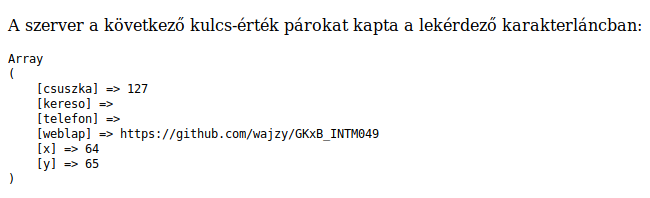
\includegraphics[width=\textwidth]{urlap6-2.png}
  \end{columns}
\end{frame}

%116
\begin{frame}
  \begin{exampleblock}{\textattachfile{urlap6.html}{urlap6.html} 
  (\textattachfile{urlap6-submit.png}{urlap6-submit.png}, \textattachfile{urlap2.php}{urlap2.php})}
    \footnotesize
    \lstinputlisting[style=HTML,linerange={9-22},numbers=left,firstnumber=9]{urlap6.html}
  \end{exampleblock}
\end{frame}

%117
\begin{frame}
  Vezérlők, amiket \emph{nem} az \texttt{input} elemmel hozunk létre:
  \begin{description}[m]
    \item[\texttt{<select>}] \hfill \\ Legördülő lista, melynek 
    bejegyzéseit \texttt{option} elemekkel adhatjuk meg. Attribútumai:
    \begin{description}[m]
      \item[\texttt{size}] \hfill \\ Ennyi elem fog látszani egyszerre 
      egymás alatt (görgethető doboz)
      \item[\texttt{multiple}] \hfill \\ Több elem is kiválasztható 
      egyszerre (Ctrl, Shift) (PHP: a \texttt{name} értéke 
      \texttt{[]}-re végződjön!)
    \end{description}
    \item[\texttt{<optgroup>}] \hfill \\ Sok lehetőség esetén 
    csoportok képzésére: \texttt{<select>} $\to$ \texttt{<optgroup>} 
    $\to$ \texttt{<option>}
    \begin{description}[m]
      \item[\texttt{label}] \hfill \\ Csoport (ki nem választható) 
      felirata
    \end{description}
  \end{description}
\end{frame}

%118
\begin{frame}
  \begin{description}[m]
    \item[\texttt{<textarea>}] \hfill \\ Hosszabb szövegek 
    megadására. Még a címkék közötti fehér karaktereket is 
    belefoglalja a vezérlő tartalmába! Attribútumok:
    \begin{description}[m]
      \item[rows] \hfill \\ Sorok száma
      \item[cols] \hfill \\ Oszlopok száma
    \end{description}
    \item[<button>] \hfill \\ Hasonló, mint \texttt{<input 
    type="button">}, de HTML/CSS formázható tartalommal.
    \begin{description}[m]
      \item[type] \hfill \\ A gomb típusa, lehet \texttt{button}, 
      \texttt{submit} és \texttt{reset}.
    \end{description}
  \end{description}
\end{frame}

%119
\begin{frame}
  \begin{description}[m]
    \item[\texttt{<output>}] \hfill \\ JavaScript számítások 
    eredményének jelölésére. Nincs látványos formázása.
    \begin{description}[m]
      \item[\texttt{for}] \hfill \\ Azon \texttt{<input>} elemek 
      \texttt{id}-i szóközzel elválasztva, melyekből kiindulva az eredmény 
      megszületett.
    \end{description}
  \end{description}
  \begin{columns}[T]
    \column{0.5\textwidth}
      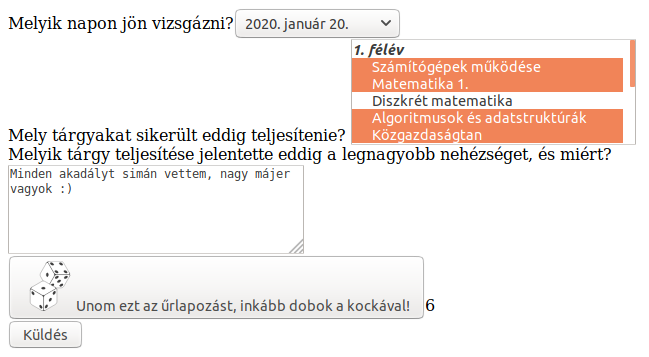
\includegraphics[width=\textwidth]{urlap7-1.png}
    \column{0.45\textwidth}
      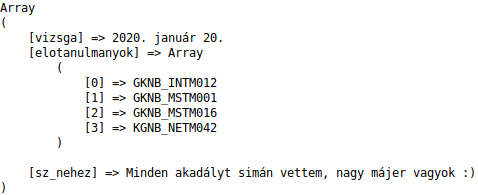
\includegraphics[width=\textwidth]{urlap7-2.png}
  \end{columns}
\end{frame}

%120
\begin{frame}
  \begin{exampleblock}{\textattachfile{urlap7.html}{urlap7.html} 
  (\textattachfile{dice.svg}{dice.svg}, \textattachfile{urlap2.php}{urlap2.php})}
    \footnotesize
    \lstinputlisting[style=HTML,linerange={9-14},numbers=left,firstnumber=9]{urlap7.html}
  \end{exampleblock}
\end{frame}

%121
\begin{frame}
  \begin{exampleblock}{\textattachfile{urlap7.html}{urlap7.html}}
    \footnotesize
    \lstinputlisting[style=HTML,linerange={15-18},numbers=left,firstnumber=15]{urlap7.html}
    \lstinputlisting[style=HTML,linerange={22-25},numbers=left,firstnumber=22]{urlap7.html}
    \lstinputlisting[style=HTML,linerange={29-31},numbers=left,firstnumber=29]{urlap7.html}
  \end{exampleblock}
\end{frame}

%122
\begin{frame}
  \begin{exampleblock}{\textattachfile{urlap7.html}{urlap7.html}}
    \footnotesize
    \lstinputlisting[style=HTML,linerange={32-40},numbers=left,firstnumber=32]{urlap7.html}
  \end{exampleblock}
\end{frame}

%123
\begin{frame}
  \scriptsize
  A mellékelt ábrának megfelelően hozzon létre egy weboldalt! Az adatokat küldje a \texttt{http://xenia.sze.hu/\textasciitilde wajzy/html/urlap2.php} címre!
  \begin{columns}[c]
    \column{0.25\textwidth}
      \begin{itemize}
        \item Az \emph{Extrák} közül többet is lehessen választani!
        \item A választható \emph{színek} legyenek: \emph{fehér}, \emph{szürke}, 
        \emph{fekete}, \emph{vörös}, \emph{kék}, \emph{sárga}. Alapértelmezetten legyen 
        kiválasztva a \emph{vörös}!
        \item A \emph{fényezés} típusa alapértelmezetten legyen 
        \emph{normál}!
      \end{itemize}
    \column{0.8\textwidth}
      \begin{exampleblock}{\small \textattachfile{urlap8.html}{urlap8.html}}
        \vspace{-.5cm}
        \begin{columns}[T]
          \column{0.45\textwidth}
            \begin{center}
              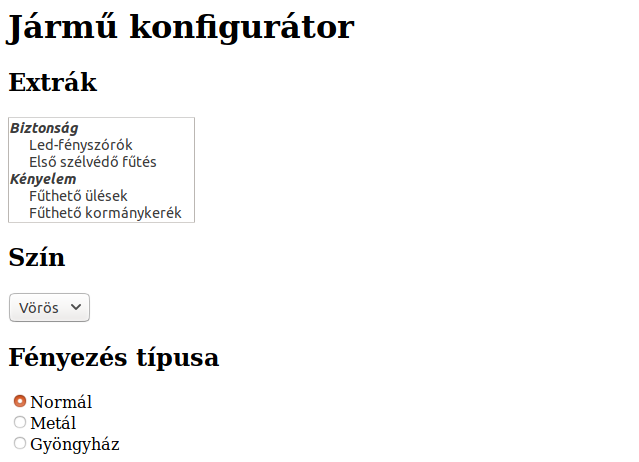
\includegraphics[width=\textwidth]{urlap8-1.png}\\
              \tiny Az oldal teteje
            \end{center}
          \column{0.45\textwidth}
            \begin{center}
              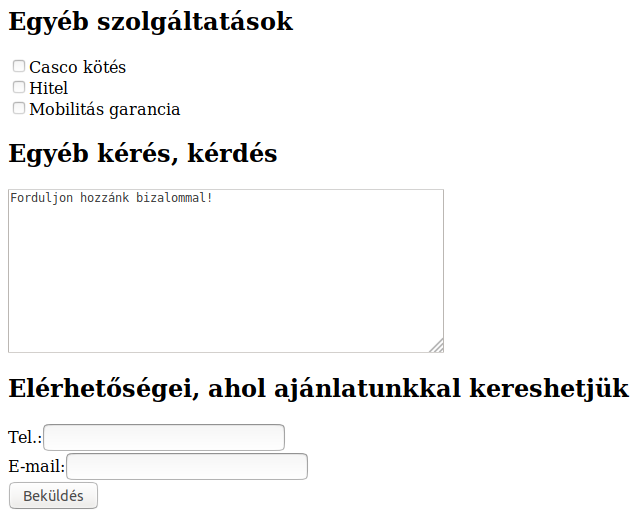
\includegraphics[width=\textwidth]{urlap8-2.png}\\
              \tiny Az oldal alja
            \end{center}
        \end{columns}
      \end{exampleblock}
  \end{columns}
\end{frame}

\subsection{Média támogatás}

%124
\begin{frame}
  A HTML5-ben beépülő modulok (pl. Flash) és akár programozás nélkül 
  lehet videót lejátszani a \texttt{<video>} elemmel (de a böngészők codec 
  támogatása hiányos). Használható formátumok:
  \begin{itemize}
    \item MP4 (video/mp4, \hiv{\href{https://caniuse.com/\#feat=mpeg4}{legjobb böngésző támogatás}})
    \item WebM (video/webm)
    \item Ogg (video/ogg)
  \end{itemize}
  Ha biztosra akarunk menni: publikálás több formátumban is.\\
  Formátumok közötti konvertálás: pl. 
  \hiv{\href{http://www.mirovideoconverter.com/}{MiroVideoConverter}}\\
  A lejátszás programozható a \hiv{\href{https://developer.mozilla.org/en-US/docs/Web/API/HTMLMediaElement}{Media API}}-val\\
\end{frame}

%125
\begin{frame}
  Ha a \texttt{<video>} elem nem támogatott egy böngészőben, a 
  címkék közötti szöveg jelenik meg. Opcionális attribútumok:
  \begin{description}[m]
    \item[\texttt{autoplay}] \hfill \\ A lejátszás azonnal indul; 
    \kiemel{nem ajánlott}, zavarhatja a felhasználót
    \item[\texttt{controls}] \hfill \\ Vezérlő gombokat jelenít meg
    \item[\texttt{width}, \texttt{height}] \hfill \\ A lejátszó 
    ablak szélessége, magassága képpontokban; \kiemel{ajánlott} megadni
    \item[\texttt{loop}] \hfill \\ Végtelenített lejátszás
  \end{description}
\end{frame}

%126
\begin{frame}
  \begin{description}[m]
    \item[\texttt{muted}] \hfill \\ Némítás
    \item[\texttt{poster}] \hfill \\ Egy kép, amit a betöltés 
    alatt / lejátszás megkezdéséig lát a felhasználó. Érték: URL
    \item[\texttt{preload}] \hfill \\ Adatfolyam betöltési módja. 
    Érték: \texttt{auto | metadata | none}.
    \item[\texttt{src}] \hfill \\ Videó forrása. \kiemel{Nem 
    ajánlott} a használata, mert csak egyetlen forrás nevezhető meg, 
    amit valószínűleg nem támogat minden böngésző. Érték: URL.
  \end{description}
\end{frame}

%127
\begin{frame}
  \begin{exampleblock}{\textattachfile{video1.html}{video1.html}}
    \footnotesize
    \lstinputlisting[style=HTML,linerange={8-13},numbers=left,firstnumber=8]{video1.html}
  \end{exampleblock}
    \begin{center}
    
\includegraphics[scale=.2]{video1.png}
  \end{center}
\end{frame}

%128
\begin{frame}
  Több adatforrás is megadható beágyazott \texttt{<source>} elemekkel, melyek 
  közül a böngésző az első támogatott formátumhoz tartozót 
  fogja választani. Attribútumok:
  \begin{description}[m]
    \item[\texttt{src}] \hfill \\ Adatforrás. Érték: URL
    \item[\texttt{type}] \hfill \\ A forrás MIME típusa.
  \end{description}
  A \texttt{<video>} elemmel történő kísérletezéshez egy 
  \hiv{\href{http://v4e.thewikies.com/}{érdekes eszköz}}.
\end{frame}

%129
\begin{frame}
  \begin{exampleblock}{\textattachfile{video2.html}{video2.html}}
    \scriptsize
    \lstinputlisting[style=HTML,linerange={8-22},numbers=left,firstnumber=8]{video2.html}
  \end{exampleblock}
\end{frame}

%130
\begin{frame}
  A videók feliratozhatóak is a \texttt{<track>} elemmel. Felirat 
  formátum: \hiv{\href{https://www.w3.org/TR/webvtt1/}{VTT}}. 
  \hiv{\href{https://www.nikse.dk/SubtitleEdit/Online}
  {Online szerkesztő}}, 
  \hiv{\href{https://subtitletools.com/convert-to-vtt-online}{átalakító}}. 
  Attribútumok:
  \begin{description}[m]
    \item[\texttt{default}] \hfill \\ Kijelölhető több feliratsáv 
    közül az alapértelmezett.
    \item[\texttt{kind}] \hfill \\ Feliratsáv típusa: 
    \texttt{captions | chapters | descriptions | metadata | 
    subtitles} (ez az alapértelmezés).
    \item[\texttt{label}] \hfill \\ Feliratsáv címkéje, pl. a 
    felirat nyelve.
    \item[\texttt{src}] \hfill \\ A felirat forrása, kötelező. 
    Érték: URL
    \item[\texttt{srclang}] \hfill \\ Felirat nyelvének ISO 639-1 
    kódja, pl. hu.
  \end{description}
\end{frame}

%131
\begin{frame}
  \begin{exampleblock}{\textattachfile{video3.html}{video3.html} 
  (\textattachfile{subtitle.vtt}{subtitle.vtt})}
    \scriptsize
    \lstinputlisting[style=HTML,linerange={8-23},numbers=left,firstnumber=8]{video3.html}
  \end{exampleblock}
\end{frame}

%132
\begin{frame}
  Feladat: készítse el a Big Buck Bunny webes lejátszóját!
  \begin{columns}[c]
    \column{0.45\textwidth}
      \begin{itemize}
        \scriptsize
        \item A videó felbontása 800x450 képpont.
        \item Poszter fotó: 
        \texttt{https://upload.wikimedia.org/wikipedia/}
        \texttt{commons/thumb/c/c5/}
        \texttt{Big\_buck\_bunny\_poster\_big.jpg/}
        \texttt{800px-Big\_buck\_bunny\_poster\_big.jpg}
        \item Két adatforrás is van, ezeket kell felajánlani: 
        \texttt{https://download.blender.org/peach/}
        \texttt{bigbuckbunny\_movies/}
        \texttt{big\_buck\_bunny\_480p\_stereo.ogg}
        és ugyanezen az útvonalon \texttt{big\_buck\_bunny\_480p\_h264.mov} 
        néven.
        \item Feliratsáv nem áll rendelkezésre.
        \item Biztosítsa a letöltés lehetőségét, ha a böngésző nem 
        támogatja a lejátszást!
      \end{itemize}      
    \column{0.45\textwidth}
      \begin{exampleblock}{\textattachfile{video4.html}{video4.html}}
        \begin{center}
          
\includegraphics[width=\textwidth]{video4.png}\\
        \end{center}
      \end{exampleblock}
  \end{columns} 
\end{frame}

%133
\begin{frame}
  Az \texttt{<audio>} elemmel lehet hangokat, zenét lejátszani. 
  Szabványos formátumok:
  \begin{itemize}
    \item MP3 (audio/mpeg, \hiv{\href{https://caniuse.com/\#feat=mp3}
    {legjobb böngésző támogatás}})
    \item Wav (audio/wav)
    \item Ogg (audio/ogg)
  \end{itemize}
  Attribútumai a méretektől eltekintve azonosak a 
  \texttt{<video>}-éival. \\
  Itt is célszerű az adatforrást beágyazott \texttt{<source>} 
  elemekkel megadni, és a lejátszást nem támogató böngészőknél 
  hibaüzenetet megjeleníteni.
\end{frame}

%134
\begin{frame}
  \begin{exampleblock}{\textattachfile{audio1.html}{audio1.html}
    (\textattachfile{dog.ogg}{dog.ogg}, 
     \textattachfile{dog.mp3}{dog.mp3})}
    \small
    \lstinputlisting[style=HTML,linerange={8-15},numbers=left,firstnumber=8]{audio1.html}
  \end{exampleblock}
  \begin{center}
    
\includegraphics[scale=.5]{audio1.png}\\
  \end{center}
\end{frame}

\subsection{Blokkszintű és soron belüli elemek}

%_
\begin{frame}
  Blokkszintű és soron belüli elemek
  \begin{itemize}
    \item A blokkszintű (\emph{block-level}) elemek mindig új sorban kezdődnek, és vízszintesen kitöltik a rendelkezésre álló helyet. Sokkal találkoztunk már:\\
    \tiny \texttt{<p>}, \texttt{<h1>}-\texttt{<h6>}, \texttt{<nav>}, \texttt{<main>}, \texttt{<article>}, \texttt{<section>}, \texttt{<header>}, \texttt{<footer>}, \texttt{<aside>}, \texttt{<address>}, \texttt{<blockquote>}, \texttt{<figure>}, \texttt{<figcaption>}, \texttt{<form>}, \texttt{<fieldset>}, \texttt{<ul>}, \texttt{<ol>}, \texttt{<li>}, \texttt{<dl>}, \texttt{<dt>}, \texttt{<dd>}, \texttt{<hr>}, \texttt{<pre>}, \texttt{<table>}, \texttt{<video>}. \normalsize 
    \item Néhánnyal ez az oktatóanyag nem foglalkozik, pl.\\ \tiny \texttt{<canvas>}, \texttt{<noscript>}. \normalsize 
    \item Egy, a későbbiekben fontos, más elemek csoportosítására (konténer) és formázására ($\to$ CSS) használt, szemantikai töltettel nem rendelkező elem: \texttt{<div>}.
  \end{itemize}
\end{frame}

%_
\begin{frame}
  \begin{itemize}
    \item A soron belüli (\emph{inline}) elemek nem kezdődnek új sorban, és csak annyi helyet foglalnak el, amennyit a tartalom mérete indokol. Sokkal találkoztunk már:\\ 
    \tiny \texttt{<a>}, \texttt{<abbr>}, \texttt{<em>}, \texttt{<strong>}, \texttt{<b>}, \texttt{<i>}, \texttt{<big>}, \texttt{<small>}, \texttt{<sup>}, \texttt{<sub>}, \texttt{<br>}, \texttt{<label>}, \texttt{<input>}, \texttt{<output>}, \texttt{<button>}, \texttt{<select>}, \texttt{<textarea>}, \texttt{<bdo>}, \texttt{<cite>}, \texttt{<q>}, \texttt{<code>}, \texttt{<var>}, \texttt{<samp>}, \texttt{<kbd>}, \texttt{<img>}, \texttt{<map>}, \texttt{<time>}. \normalsize
    \item Néhány, főleg elavult vagy más területekre átvezető elemmel ez az oktatóanyag nem foglalkozik, pl.\\ \tiny \texttt{<acronym>}, \texttt{<object>}, \texttt{<tt>}, \texttt{<script>}. \normalsize
    \item Egy, a későbbiekben fontos, soron belüli részek (adatok, pl. szöveg és más soron belüli elemek) megjelölésére és formázására ($\to$ CSS) használt, szemantikai töltettel nem rendelkező elem: \texttt{<span>}.
  \end{itemize}
\end{frame}

%_
\begin{frame}
  A blokkszintű és soron belüli elemek megkülönböztetése a HTML 4.x szabványok sajátossága volt. Ezeket leváltották a HTML5 \hiv{\href{https://html.spec.whatwg.org/multipage/dom.html\#content-models}{tartalmi kategóriái}}, de bizonyos párhuzamosságok továbbra is megfigyelhetőek (pl. \emph{inline} $\to$ \emph{phrasing content}), és a régi fogalmak a korszerű oldalak készítésénél is többnyire egyértelműen és kifejező módon használhatóak. 
\end{frame}

\subsection{Összefoglaló feladatok}

\newcounter{feladatSzamlalo}

%_
\begin{frame}
  Fejlessze tovább a Wiki által ihletett, CSS-t ismertető weboldalt!
  \begin{columns}[c]
    \column{0.25\textwidth}
      \begin{exampleblock}{\textattachfile{cssFormazott.html}{cssFormazott.html}, \textattachfile{css.css}{css.css}}
        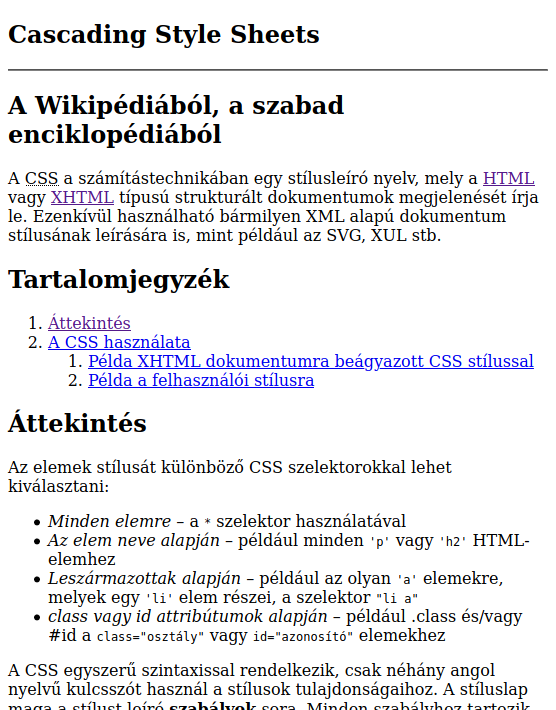
\includegraphics[width=\textwidth]{css1.png}
      \end{exampleblock}
    \column{0.75\textwidth}
      \begin{enumerate}
        \footnotesize
        \item Induljon ki a korábban létrehozott \textattachfile{../html2/css.html}{css.html} fájlból! Ha kell, egészítse ki a HTML kódot új (pl. \texttt{class}, \texttt{id}) attribútumokkal!
        \item Kapcsolja ezt össze egy \texttt{css.css} nevű stíluslappal, amit készítsen el az alábbi pontoknak megfelelően!
        \item A címsorok betűtípusa legyen \emph{Linux Libertine}, ennek hiányában \emph{Georgia}, \emph{Times}, de legalább valamilyen talpas betűkészlet!
        \item A bekezdések betűmérete legyen 14 nyomdai pont, a sortávolság legyen 1,5-szeres!
        \item Az első szintű címsor betűmérete legyen a bekezdések betűméretének 1,8-szerese, a második szintűké 1,5-szeres, a harmadik szintűeké pedig 1,2-szeres! Ez utóbbit szedje félkövér betűkkel!
        \item A hiperhivatkozások csak akkor legyenek aláhúzva, ha éppen felettük van az egér!
        \setcounter{feladatSzamlalo}{\theenumi}
      \end{enumerate}
  \end{columns}
\end{frame}

%_
\begin{frame}
  \begin{columns}[c]
    \column{0.25\textwidth}
      \begin{exampleblock}{\textattachfile{cssFormazott.html}{cssFormazott.html}, \textattachfile{css.css}{css.css}}
        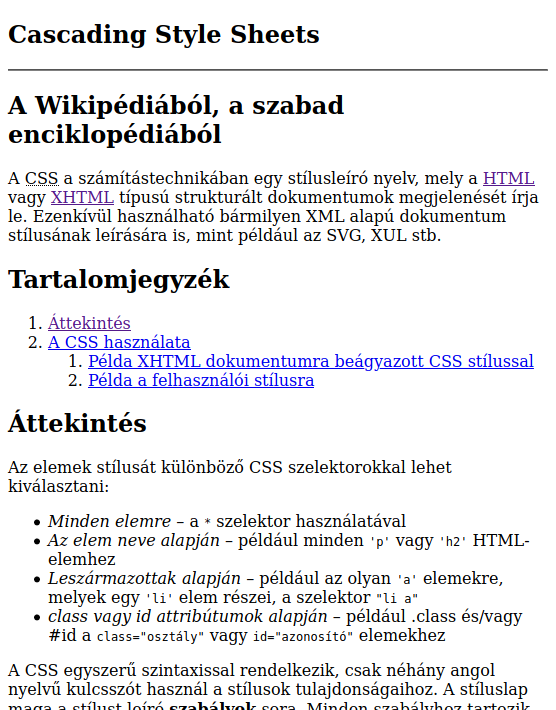
\includegraphics[width=\textwidth]{css1.png}
      \end{exampleblock}
    \column{0.75\textwidth}
      \begin{enumerate}
        \setcounter{enumi}{\thefeladatSzamlalo}
        \item A tartalomjegyzéket vegye körül 1 képpont széles, folytonos, szürke színű szegéllyel!
        \item A háttérszín is legyen szürke, melynek minden RGB komponense 240 értékű!
        \item Maga a tartalomjegyzék ne legyen szélesebb, mint amit a tartalma indokol!
        \item A jobb oldalon állítsa 20 képpontra a kitöltést!
        \item A ,,Tartalomjegyzék'' felirat legyen középre igazítva!
        \item A felsorolások bal oldali kitöltése legyen 20 képpont!
        \item A számozás szintenként folytonos legyen, a minta szerint!
        \setcounter{feladatSzamlalo}{\theenumi}
      \end{enumerate}
  \end{columns}
\end{frame}

%_
\begin{frame}
  \begin{columns}[c]
    \column{0.25\textwidth}
      \begin{exampleblock}{\textattachfile{cssFormazott.html}{cssFormazott.html}, \textattachfile{css.css}{css.css}}
        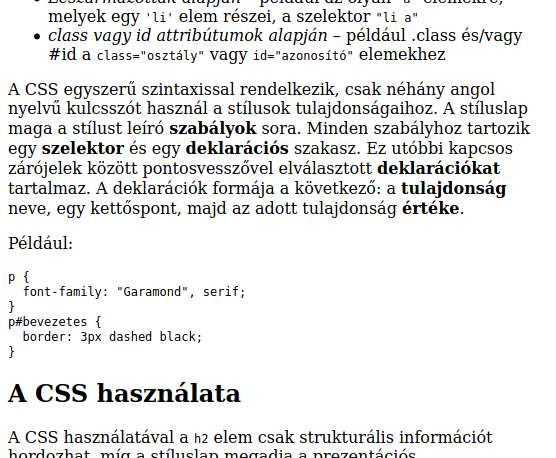
\includegraphics[width=\textwidth]{css2.png}
      \end{exampleblock}
    \column{0.75\textwidth}
      \begin{enumerate}
        \setcounter{enumi}{\thefeladatSzamlalo}
        \small
        \item A programkódok, akár egy soron belül helyezkednek el, akár előformázott szövegként, kapjanak világosszürke hátteret, melynek RGB összetevői 16-os számrendszerben rendre \texttt{f8}, \texttt{f9} és \texttt{fa}!
        \item A szegélyek 1 képpont széles, folytonos vonalak, melyek színének komponensei: \texttt{ea}, \texttt{ec} és \texttt{f0}!
        \item A szöveg legyen 14 képpont méretű, félkövér betűkkel szedett!
        \item Ha a kód soron belül található, a szegélye legyen 2 képpont sugarú lekerekítéssel ellátva, továbbá fent és lent 1-1, a két oldalon pedig 4-4 képpont belső kitöltéssel rendelkezzen!
        \item Ezzel szemben az előformázott szövegeknek minden oldalán hagyjon akkora kitöltést, mint amekkora az alapértelmezett betűméret!
        \setcounter{feladatSzamlalo}{\theenumi}
      \end{enumerate}
  \end{columns}
\end{frame}

%_
\begin{frame}
  \begin{columns}[c]
    \column{0.25\textwidth}
      \begin{exampleblock}{\textattachfile{cssFormazott.html}{cssFormazott.html}, \textattachfile{css.css}{css.css}}
        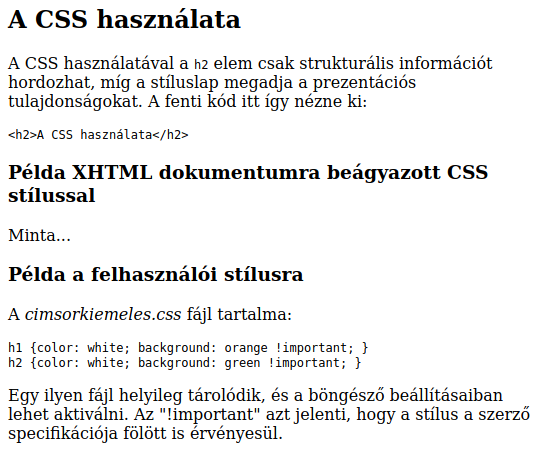
\includegraphics[width=\textwidth]{css3.png}
      \end{exampleblock}
    \column{0.75\textwidth}
      A szintaktikai kiemeléssel ellátott CSS forrásszövegben
      \begin{enumerate}
        \setcounter{enumi}{\thefeladatSzamlalo}
        \item az elemnevek, tulajdonságok és kulcsszavak színe legyen zöld,
        \item az \texttt{id} legyen kék,
        \item a mértékegység és a karakterlánc típusú adat legyen piros,
        \item a mennyiség pedig szürke!
      \end{enumerate}
  \end{columns}
\end{frame}


\end{document}
